\documentclass{article}

\usepackage{graphicx}
\usepackage{amsmath}

\usepackage{listings}
\lstset{
escapeinside={(*}{*)},
frame=single
}


\title{A Genetic Algorithm Approach to Graph Coloring \\
       \large CSE 591 Spring 2018 Project One}
\author{Kirtus Leyba}

\begin{document}
\maketitle

\section{Introduction}

    The Graph Coloring Problem is defined as completely labeling the vertices of a Graph $(G = (V,E))$ such that no edges connect two vertices of the same discrete label, or "color". The graph coloring problem presents many challenges. For instance, solutions will vary widely for a given number of colors on topologically diverse graphs, and solutions will again be diverse for a different number of colors on a single graph. This diverse solution space and hard computational problem suggests that genetic algorithms (GAs) might be effective tools for generating graph coloring solutions. This project investigates this potential and explores some graph attributes that may play a role in the effectiveness of genetic algorithms on this problem.

\section{The Genetic Algorithm}

	\subsection{Design}
	The genetic algorithm implementation for this project follows many of the standards of genetic algorithms. Chromosomes are defined to be strings of some encoding that maps onto a search space. Generally, these chromosomes can be thought of as bit strings, and each information carrying cell in the string can be thought of as a gene. Three primary operators are defined to act on individual chromosomes or populations: \textbf{selection}, \textbf{crossover}, and \textbf{mutation}. Put very briefly, selection determines which individuals in a population pass on genetic information, crossover distributes genetic information from multiple parents to multiple offspring, and mutation introduces steady, random genetic changes. Iteratively applying these operators across generations will hopefully result in finding the most fit solutions in the search space.\par

	To confirm that this genetic algorithm could correctly evolve to a fit solution, a max ones problem was solved as a dummy challenge. In max ones, the GA simply attempts to convert the entire population into bit strings full of only ones. For example, a bit string $\{1111\}$ would be the most fit and $\{0000\}$ would be the least fit. Using a simple, 1 counting fitness function, the GA quickly solved this problem in less than 5 generations.

	\subsection{Implementation}
	The genetic algorithm was implemented in Java to take advantage of portabillity and encapsulation. Creating a general, abstract class, and then making specific child instances lends itself well to genetic algorithm design, as modularity enables fast iteration and testing on different ideas. A general genetic algorithm frame work can easily be adjusted to work with various encodings, and thus can be used to solve many problems. Java's abstraction level led to fast development in this regard.\par

	The particulars of the GA used are as follows. Tournament selection was used with a \textbf{tournament size} of 2 and a \textbf{selection probability} of 0.85, a simple \textbf{2 point crossover} operator was chosen, and a random gene was flipped, with \textbf{mutation probability} 0.001, to another random legal value (application dependent) for mutation.\par

\section{Finding Graph Colorings}

	A simple encoding of integers was used for the graph coloring problem. To ensure that a random individual was truly uniformly chosen from the search space, a single chromosome was represented as an array of integers equal in length to the number of nodes. Each index corresponded to the coloring of that vertex in that solution for the graph. Two fitness functions were used: a direct fitness function that found the fraction of correct edges to total edges (eqn. 1 ), and a balanced fitness function (eqn. 2 ) that targeted colorings where each color was as evenly represented as possible.\par

	\begin{equation} \label{eqn:standardFitness}
	F(C(G)) = \frac{\sum_{i,j\in E}\delta(i,j)}{m}
	\end{equation}

	\begin{equation} \label{eqn:balance}
	F(C(G)) = \frac{\sum_{i,j\in E}\delta(i,j)}{m{k^k}}\prod_{i=1}^{k}\frac{|V_i|}{n}
	\end{equation}

	Figure \ref{fig:fitness} shows that, for the standard fitness function, some graphs were more difficults for the GA than others. Graphs with many nodes and high degree particulary seemed challenging. This consideration is investigated more below. As a stochastic method, genetic algorithms do not always perform the same, run to run. To determine the importance of random number generation in a run, figure \ref{fig:standard} shows the fitness across many runs, accompanied by the region of standard deviation around the mean. It can be seen that the results are very close together. Thus, it is safe to say that the genetic algorithm's effectiveness is not limited directly by the stochastic nature of each run.

	\begin{figure}
		\centering
		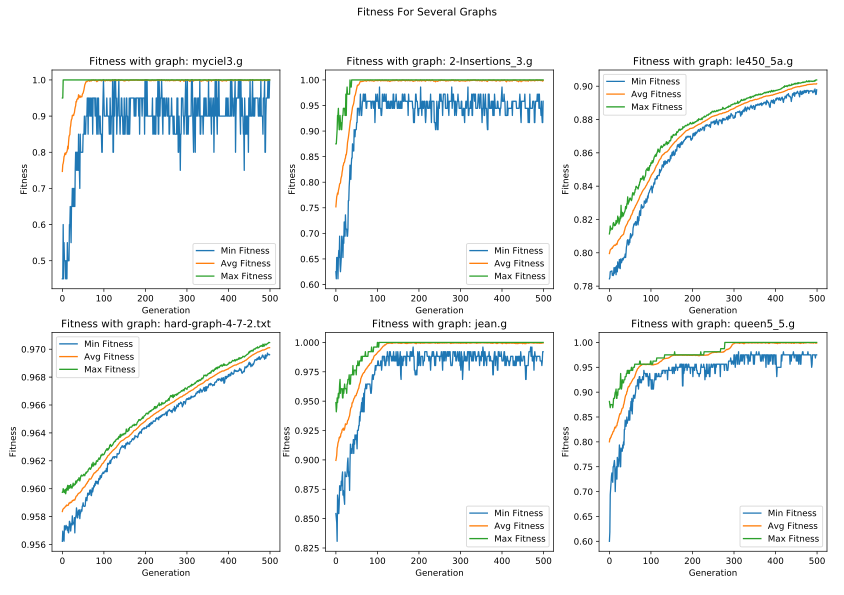
\includegraphics[width=12cm, height=8cm]{FitnessFigure.png}
		\caption{The performance of the genetic algorithm on multiple graphs}
		\label{fig:fitness}
	\end{figure}

	\begin{table}[]
	\centering
	\caption{Correctness with standard and balanced fitness functions}
	\label{correct}
	\begin{tabular}{llll}
	\hline
	Standard Fitness &             &                     &         \\ \hline
	Graph            & Max Fitness & Generation Achieved & Correct \\ \hline
	2-Insertions\_3  & 1.0         & 53                  & Yes     \\ \hline
	hard-graph-4-7-2 & 0.97        & 499                 & No      \\ \hline
	jean             & 1.0         & 397                 & Yes     \\ \hline
	le450\_5a        & 0.906       & 487                 & No      \\ \hline
	myciel3          & 1.0         & 1                   & Yes     \\ \hline
	queen5\_5        & 1.0         & 234                 & Yes     \\ \hline
	Balanced Fitness &             &                     &         \\ \hline
	2-Insertions\_3  & 0.996       & 78                  & Yes     \\ \hline
	hard-graph-4-7-2 & 0.952       & 488                 & No      \\ \hline
	jean             & 0.97        & 387                 & No      \\ \hline
	le450\_5a        & 0.896       & 497                 & No      \\ \hline
	myciel3          & 0.944       & 1                   & Yes     \\ \hline
	queen5\_5        & 0.919       & 99                  & No      \\ \hline
	\end{tabular}
	\end{table}

	\begin{figure}
		\centering
		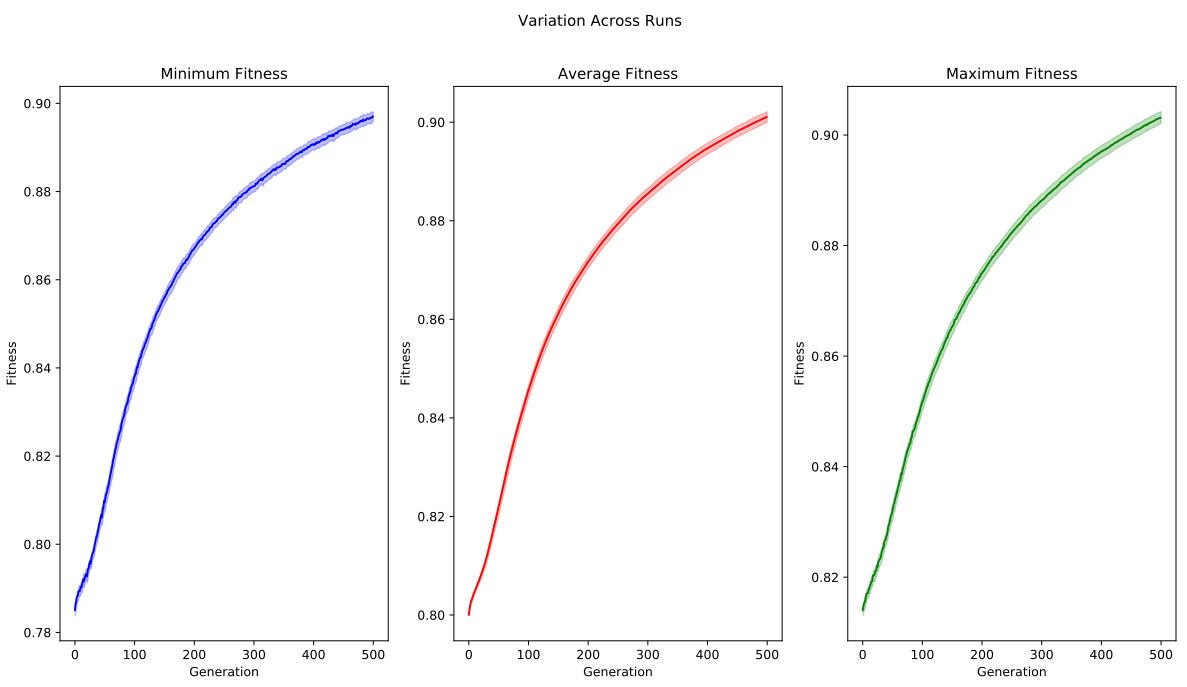
\includegraphics[width=12cm,height=6cm]{standard.png}
		\caption{The variation of the genetic algorithm across many runs}
		\label{fig:standard}
	\end{figure}

\section{Neutrality of Graph Colorings}

	In order to develop an understanding of what graphs are difficult for the genetic algorithm to solve, the Erd\H{o}s-R\'{e}nyi model was used to generate graphs with an expected average degree. Figure \ref{fig:erdos} is an example of such a random graph with an expected average degree of 1.25.\par

	\begin{figure}
		\centering
		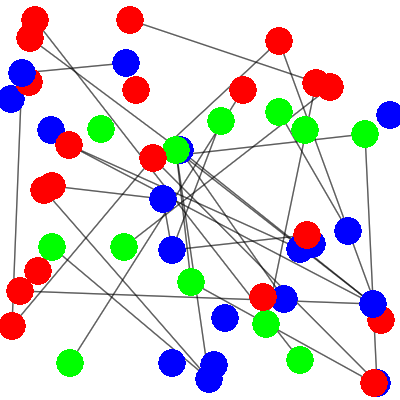
\includegraphics[scale = 0.25]{erdos.png}
		\caption{An Erd\H{o}s-R\'{e}nyi Graph with average degree of 1.25}
		\label{fig:erdos}
	\end{figure}

	One might expect that graphs with higher degree will be more difficult to solve, as each vertex will have to be compared against a higher number of neighbors on average. The following two figures, \ref{fig:degree} and \ref{fig:neutral}, illustrate this idea through experiment. The max fitness achieved over the same number of generations, and averaged across many runs, goes into steep decline for graphs with higher degree. This suggests that the GA is searching in a large search space with few fit solutions, and much fewer completely correct solutions. As shown in figure \ref{fig:neutral}, the neutrality of the graph exhibits this relationship. Graph neutrality, or the measure of other correct colorings to a graph, given an initial valid coloring, illuminates the effect that degree has on the search space. This result could be an indicator that the graph coloring problem has challenges insurmountable to GAs. Covnersely, it is possible that some diversity preference such as fitness sharing, distance penalties, or speciation could dramatically improve a GAs performance on the graph coloring problem. This is left as a future exploration beyond the scope of this project.

	\begin{figure}
		\centering
		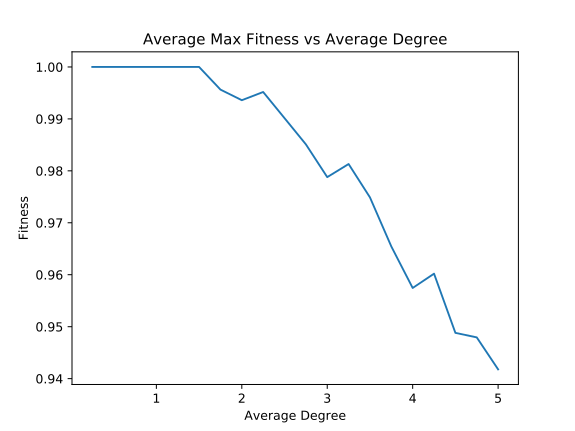
\includegraphics[scale = 0.5]{degree.png}
		\caption{The effect of degree on max fitness}
		\label{fig:degree}
	\end{figure}
	\begin{table}[]
	\centering
	\caption{Some Valid Colorings and Neutrality}
	\label{valid}
	\begin{tabular}{lllll}
	\hline
	Graph File      & Original Coloring                     & Neutrality          &  &  \\ \hline
	myciel3         & 30221333010                           & 0.4090909090909091  &  &  \\ \hline
	2-Insertions\_3 & 3000032212310133213011020322321211120 & 0.43243243243243246 &  &  \\ \hline
	queen5\_5       & 1402332040342140210313421             & 0.2                 &  &  \\ \hline
	\end{tabular}
	\end{table}

	\begin{figure}
		\centering
		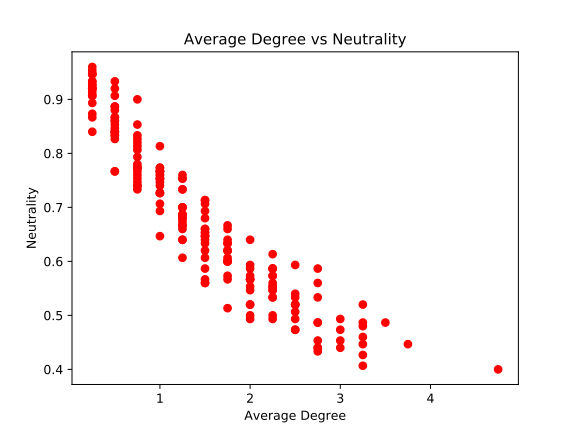
\includegraphics[scale = 0.5]{neutral.png}
		\caption{The neutrality of solutions with various average degree}
		\label{fig:neutral}
	\end{figure}

\section{Discussion and Conclusion}
	The graph coloring problem is a problem that has attractive facets when it comes to genetic algorithms as well as some clear challenges. Through this project it has been shown that graphs with low neutrality stand as particularly difficult tasks to tackle for genetic algorithms. The importance of the search space landscape in regards to the success of genetic algorithms is evident in this particular problem. The neutrality based analysis would be worthwhile in other genetic algorithm implementations to assist in directing future experiments.

\section{Appendix}
	\subsection{Graph Coloring Solutions}

	Included here are valid colorings that were found for the various input graphs.

	\begin{table}[h!]
	\centering
	\caption{Valid Colorings}
	\label{colo}
	\begin{tabular}{ll}
	\hline
	Graph           & Coloring                                                                      \\ \hline
	queen5\_5       & 1402332040342140210313421                                                     \\ \hline
	myciel3         & 30221333010                                                                   \\ \hline
	jean            & 01904852433611453709718056246935219871352971747470503755251014076867389526429 \\ \hline
	2-Insertions\_3 & 3000032212310133213011020322321211120                                         \\ \hline
	\end{tabular}
	\end{table}

	\subsection{Source Code Repository}

\end{document}
